\section{Introduction}\label{introduction}

\subsection{Motivation}\label{motivation}

A single aggregate performance summary cannot by itself show where a
workflow remains reliable or where it fails across controlled changes in
observational difficulty.

Astronomical photometry and source-extraction workflows have been
evaluated with controlled simulations, injected sources, and
survey-level validation. Comparisons on simulated images can expose
condition-dependent behavior, including degradation in crowded or
overdense scenes \cite{ref1}. Injection frameworks such as HSC SynPipe
place synthetic sources into real survey images and have revealed
blending-dependent photometric caveats \cite{ref2}. Foundational tools
such as SExtractor provide automated source detection, deblending,
measurement, and classification capabilities \cite{ref3}, while large
survey releases such as Gaia EDR3 include dedicated photometric
validation and systematic-quality assessment \cite{ref4}. End-to-end
simulators such as PhoSim provide another route for studying pipeline
behavior and systematics, while still requiring comparison with real
data to establish fidelity in observational use \cite{ref5}. The AMPV
study is designed around that gap in evaluation structure: instead of
treating validation as a single ranking problem, it maps workflow
behavior across a frozen stress grid and retains the cell-level evidence
needed to identify reliability boundaries.

Astronomical image simulation and injection-based validation also
provide mature precedents for testing image-analysis systems. GalSim
provides a general-purpose, high-precision framework for rendering
synthetic astronomical sources \cite{ref8}. Survey pipelines have been
characterized by inserting synthetic sources into observational images:
HSC SynPipe propagates injected objects through the HSC processing chain
\cite{ref2}, while Balrog uses large-scale injections into DES
single-epoch images to sample selection and photometric biases and the
survey transfer function \cite{ref9}. For task-specific algorithm
evaluation, the Blending ToolKit combines simulated blended-galaxy
images, standardized algorithm interfaces, and common metrics to support
principled comparisons of detection and deblending methods \cite{ref10}.
AMPV is positioned alongside, rather than prior to, these approaches.
Its emphasis in the present study is a matched compound-contamination
stress grid with preserved stochastic identities, explicit separation of
blind and privileged-information workflow classes, and cell-resolved
reliability and operational-vulnerability surfaces used to report
boundaries only on the tested grid.

The present experiment uses a controlled synthetic environment so that
ground truth, perturbation strength, and repeated scene realization can
be fixed explicitly. \cite{ref5} This makes it possible to separate
changes in workflow output from changes in the underlying stochastic
realization and to preserve a reproducible audit trail from scene
generation through numerical summary.

\subsection{From aggregate comparison to reliability
mapping}\label{from-aggregate-comparison-to-reliability-mapping}

AMPV is framed here as a validation methodology rather than as an
additional photometric estimator. The objects being evaluated are
workflows A--E; AMPV supplies the experimental design, matched-scene
structure, numerical ledger, and boundary-oriented interpretation used
to assess them.

The frozen V2 design crosses five reference-contrast levels with three
contamination levels and evaluates every workflow on the same matched
scenes. This structure supports two complementary views of performance:
continuous error behavior and a threshold-based vulnerability indicator.
Together, those views describe where error remains small, where
vulnerability becomes nonzero or increases, and how those patterns
depend on the tested stress coordinates.

\subsection{Relationship to CAPS}\label{relationship-to-caps}

AMPV and CAPS serve different roles in the present work. AMPV is the
general validation methodology used to organize stress testing,
reliability mapping, and boundary analysis. CAPS is a controlled
synthetic implementation environment that can support such experiments.
The V2 production used in this manuscript was independently realized,
audited, and canonically frozen within the AMPV V2 project tree; the
earlier CAPS V1 production outputs are not used as the canonical
evidence for the present results.

This distinction is important because the scientific contribution of the
present study is not a renamed workflow or a simple continuation of an
earlier ranking exercise. The emphasis is the reproducible methodology
for characterizing reliability across controlled perturbation space.

\subsection{Study objectives}\label{study-objectives}

The present study has four objectives:

\begin{enumerate}
\def\labelenumi{\arabic{enumi}.}
\tightlist
\item
  to define and execute a frozen matched-scene stress grid over
  reference contrast and contamination level for workflows A--E in the
  primary comet-like family, with a separately frozen blind-workflow
  A/B/C/E extension in the compact-PSF family;
\item
  to quantify both continuous error behavior and threshold-defined
  vulnerability at the cell level rather than relying only on pooled
  summaries;
\item
  to identify descriptive reliability boundaries while preserving
  workflow information-class distinctions, including the diagnostic role
  of privileged-information workflow D; and
\item
  to establish a fully traceable production-to-ledger-to-canonical
  workflow so that every manuscript number can be linked back to frozen
  V2-native evidence.
\end{enumerate}

The present study is single-fidelity but now contains two separately
versioned controlled synthetic task families. The canonical
\texttt{COMET\_LIKE\_PRIMARY} experiment is retained unchanged, and a
pre-registered \texttt{COMPACT\_PSF\_PRIMARY} extension tests whether
the AMPV reliability-mapping structure remains informative after a
material change in source morphology and estimand. Multi-fidelity
dependence remains outside the evidence supported by the current study.

\begin{figure}[htbp]
\centering
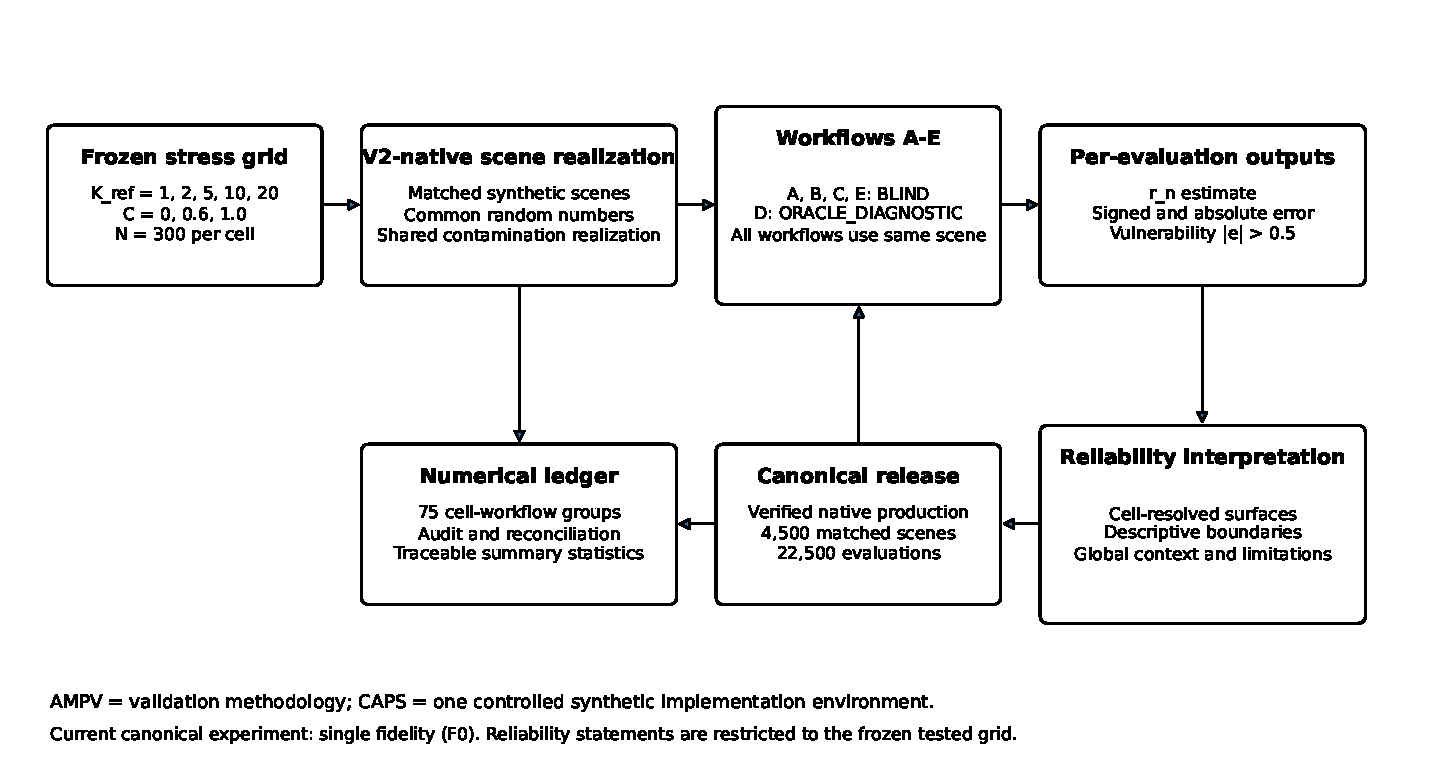
\includegraphics[width=0.88\linewidth]{figures/FIGURE_1_AMPV_FRAMEWORK.pdf}
\caption{AMPV validation framework.}
\label{fig:framework}
\end{figure}
\subsection{Scope of external context}\label{scope-of-external-context}

External context is limited to source-level-audited literature.
Prior-art statements are restricted to controlled simulation and source
injection, photometric validation, source-extraction comparison,
common-random-number methodology, and validation-domain framing
supported by Refs.
\cite{ref1,ref2,ref3,ref4,ref5,ref6,ref7,ref8,ref9,ref10}. Claims about
the present AMPV results remain grounded in the frozen V2 evidence
chain.

\section{Methods}\label{methods}

\subsection{AMPV validation design and statistical
unit}\label{ampv-validation-design-and-statistical-unit}

AMPV is used here to map workflow reliability under controlled compound
contamination. The experiment contains 300 base stochastic sample
identities. Each identity is propagated through 15 condition cells
formed by five reference-contrast levels,
\(\kappa_{\rm ref}=1,2,5,10,20\), crossed with three contamination
levels, \(C=0,0.6,1.0\). This produces 4,500 condition-specific scene
instances. Each scene instance is evaluated by workflows A--E, giving
22,500 workflow evaluations and 75 cell--workflow groups with 300
evaluations per group. The task family is \texttt{COMET\_LIKE\_PRIMARY}
at fidelity level \texttt{F0}.

The same sample identity preserves \(r_n\), interference seeds, and the
unscaled structured-contamination realization across all 15 cells. Thus
the 4,500 condition-specific instances are not treated as 4,500
statistically independent base scenes. This common-random-number design
permits paired comparisons across stress conditions and workflows while
reducing variation due solely to unrelated stochastic draws.

\subsection{Synthetic signal and compound
contamination}\label{synthetic-signal-and-compound-contamination}

The implemented comet-like source is generated on a \(256\times256\)
pixel image. The central nucleus is represented by a normalized Gaussian
component with \(\sigma=1.5\) pixels and is combined with a radial coma
component proportional to \(r_n^2/\rho^2\) after the implemented
central capping and normalization. The canonical benchmark uses a
nucleus fraction of 0.3 and a coma fraction of 0.7. This construction is
an intentionally controlled synthetic task and is not presented as a
complete physical radiative-transfer model.

Compound interference contains six implemented families: I1, sky
gradient/spatial mottling/background galaxies; I2, a dust jet and
anti-solar tail; I3, sparse cosmic-ray-like events; I4, field-star
Gaussian PSFs; I5, low-frequency detector baseline drift; and I6,
Gaussian readout noise. The structured I1--I5 realization is shared for
a given sample identity and scaled by \(C\), whereas I6 is retained
separately. The realized \(r_n\) values in the production span
0.310041--4.988671.

\subsection{Reference-contrast
calibration}\label{reference-contrast-calibration}

Reference contrast is controlled through a source-gain calibration. For
the reference regime, \(r_n=1\) km and the clean source flux is measured
in a 30-pixel aperture. The reference noise denominator is the I6
readout-noise standard deviation multiplied by the square root of the
aperture pixel count. For each target \(\kappa_{\rm ref}\), source
gain is selected so that the reference clean-aperture flux attains the
requested contrast. The resulting gains for
\(\kappa_{\rm ref}=1,2,5,10,20\) are 13.9532646896, 27.9065293792,
69.766323448, 139.532646896, and 279.065293792, respectively. The same
gain is used across the three contamination levels at a given target
contrast. The production also records the realized sample-specific
contrast separately from the configured \(\kappa_{\rm ref}\).

\subsection{Photometric workflows and information
constraints}\label{photometric-workflows-and-information-constraints}

Workflow A is a blind 30-pixel-radius aperture sum with no background
subtraction. Workflow B is blind aperture photometry using a 30-pixel
circular aperture and a fixed 50--90 pixel annulus; the annular mean is
used for background subtraction. Workflow C is blind aperture photometry
with the same aperture and background ring but uses a deterministic
RANSAC-style background estimator (seed 20260814, 200 iterations, sample
size 30, and an inlier threshold of \(0.2\\,\sigma\) of the background
pixels).

Workflow D is an \texttt{ORACLE\_DIAGNOSTIC}, not an
information-equivalent blind estimator. It uses the true \(r_n\) to
select an adaptive background annulus with inner radius
\(\max[\lceil 11r_n\rceil,35]\) pixels, subject to image-geometry
limits, a 40-pixel annulus width, and median background estimation. It
is therefore interpreted as a privileged-information diagnostic
reference.

Workflow E is blind model fitting with a circular two-dimensional
Gaussian plus constant background on a local image patch. The
least-squares parameters are source center, amplitude, Gaussian width,
and background; an analytic Jacobian is used, the Gaussian width is
bounded to 1--20 pixels, and the optimization limit is 120 function
evaluations. Fitted flux is \(2\pi |A|\sigma^2\).

Each workflow has a separate noiseless calibration curve based on 40
log-spaced \(r_n\) values from 0.1 to 10 km. Measured flux is mapped
back to \(r_n\) by log-flux interpolation. Calibration is constructed
separately for each workflow and source-gain level.

\subsection{Pre-registered compact-PSF extension}
\label{pre-registered-compact-psf-extension}

A second controlled family, \texttt{COMPACT\_PSF\_PRIMARY}, was
pre-registered and executed as a separately versioned extension after
the comet-like production had been frozen. It contains 300 base
identities crossed with the same five reference-contrast targets and
three contamination levels. Because no scientifically meaningful
privileged-information analogue of workflow D was identified before
production, the extension evaluates blind workflows A, B, C, and E,
giving 18,000 workflow evaluations.

The source is a centered circular Gaussian PSF with independently
sampled width \(\sigma_{\rm PSF}=1.5\text{--}4.0\) pixels and integrated
truth flux \(F_{\rm true}\). A two-dimensional Latin-hypercube design
(seed 20261003) samples PSF width and a narrow intrinsic-amplitude factor
of 0.8--1.2. The comet-specific dust-jet/tail interference I2 is not
reused. It is replaced, before outcome generation, by I2P: a
task-neutral asymmetric elliptical local contaminant with geometry and
amplitude fixed relative to a reference signal scale and independent of
sample \(F_{\rm true}\) and \(\sigma_{\rm PSF}\). The remaining
stress construction preserves matched sample identities across
conditions.

For this family, workflows A--C retain the same aperture/background
definitions, whereas workflow E fits the circular Gaussian plus constant
background. The estimand is integrated flux, so relative error is
\((F^{\rm est}-F_{\rm true})/F_{\rm true}\). A clean-domain audit
showed only numerical-precision-level error for A--C and E, so no
post-hoc calibration surface was introduced. The production and
statistical analysis were frozen before scientific interpretation; the
latter used 2,000 sample-identity bootstrap replicates with seed
20261004. The same primary \(\tau=0.5\) vulnerability definition and
the same threshold-sensitivity grid were retained.

\subsection{Error quantities and operational vulnerability
criterion}\label{error-quantities-and-operational-vulnerability-criterion}

Signed relative error is defined with the family-specific estimand. For
\texttt{COMET\_LIKE\_PRIMARY},
\[
e=(r_n^{\rm est}-r_n^{\rm true})/r_n^{\rm true},
\]
whereas for \texttt{COMPACT\_PSF\_PRIMARY},
\[
e=(F^{\rm est}-F_{\rm true})/F_{\rm true}.
\]
In both families, absolute error is \(|e|\). Continuous error is the
primary measure of estimation behavior. The predefined vulnerability indicator
uses \(|e|>\tau\) with the primary frozen operational threshold
\(\tau=0.5\), corresponding to a 50\% relative-error cutoff. This
threshold is not treated as a universal astronomical standard; its
robustness is examined by sensitivity analyses at
\(\tau=0.25,0.4,0.5,0.6,0.75,\) and \(1.0\).

\subsection{Paired uncertainty and robustness
analyses}\label{paired-uncertainty-and-robustness-analyses}

Uncertainty analyses use the 300 sample identities within each task
family as the resampling units. A cluster-bootstrap replicate samples
these identities with replacement and carries each selected identity's
complete cross-condition and cross-workflow block within that family,
preserving the matched-design dependence. The comet-like analysis used
2,000 replicates with fixed seed 20261002; the separately frozen
compact-PSF analysis used 2,000 replicates with fixed seed 20261004.
These analyses provide 95\% intervals for cell-level median absolute
error, median signed error, vulnerability, and paired contrasts. In the
comet-like family, blind-workflow contrasts are evaluated within matched
\((\kappa_{\rm ref},C,\mathrm{sample\\ id})\) instances and workflow D
is kept separate because of its oracle information class. The compact-PSF
extension contains only blind workflows A, B, C, and E.

Workflow E has complete optimization diagnostic records for all 4,500
evaluations. The optimizer reports \texttt{success=True} for 4,497
evaluations and \texttt{success=False} with status 0 for three. The
production validity rule classified computational failure on exception
rather than optimizer status alone. A sensitivity analysis therefore
recomputed affected summaries after excluding these three cases without
altering their canonical validity labels.

\subsection{Reproducibility and
provenance}\label{reproducibility-and-provenance}

For each task family, the experimental design, seed namespace, workflow
definitions, and stress grid were frozen before that family's production.
The original comet-like canonical release was not modified when the
separately versioned compact-PSF extension was added. Numerical summaries
and figures were generated from the corresponding verified production
rows and audited derived-analysis records without altering either
production output. Detailed hashes, audit gates,
and engineering provenance are retained in the reproducibility archive
rather than repeated in the scientific narrative.

\subsection{Ethical applicability and AI-assisted
workflow}\label{ethical-applicability-and-ai-assisted-workflow}

The present work is a computational validation study based on synthetic
astronomical scenes and simulation outputs. The AMPV V2 evidence chain
contains no human-participant, animal-subject, clinical-trial, or
personally identifiable data. On that project-evidence basis,
institutional human/animal research approval and informed consent are
not applicable to the current study scope. \textbf{{[}AUTHOR
CONFIRMATION REQUIRED BEFORE SUBMISSION{]}}

ChatGPT (OpenAI) was used as an assistive tool during manuscript
preparation and reproducibility-workflow development. Its use included
language editing; drafting and reviewing Python, PowerShell, and LaTeX
workflow scripts; organizing provenance and audit records; supporting
literature-audit and citation-workflow organization; and assisting with
figure-layout and manuscript-assembly tasks. AI assistance did not
replace the AMPV V2 numerical evidence chain. The authors remain
responsible for independent verification of scientific content, source
use, code execution records, numerical results, interpretations, and the
final manuscript text. ChatGPT is not an author.

\section{Results}\label{results}

The primary comet-like analysis contains 300 base stochastic sample
identities propagated through 15 condition cells, yielding 4,500
condition-specific scene instances and 22,500 workflow evaluations
organized into 75 cell--workflow groups. Its grid comprises five
reference-contrast levels
(reference contrast = 1, 2, 5, 10, 20), three contamination
levels (\texttt{C\ =\ 0,\ 0.6,\ 1.0}), and workflows A--E. The
comet-like values reported in the following subsections are derived from
the verified canonical release and audited numerical ledger; the
compact-PSF extension is reported separately from its independently
frozen production.

\subsection{Global descriptive behavior across the frozen
grid}\label{global-descriptive-behavior-across-the-frozen-grid}

Across the full frozen grid, the workflow-level summaries were:

\begin{itemize}
\tightlist
\item
  Workflow A: N=4500, median absolute error=0.019, IQR=0.0051--0.073,
  median signed error=0.012, vulnerability rate=5.5\%.
\item
  Workflow B: N=4500, median absolute error=0.015, IQR=0.0040--0.060,
  median signed error=0.0057, vulnerability rate=4.8\%.
\item
  Workflow C: N=4500, median absolute error=0.061, IQR=0.016--0.232,
  median signed error=8.852e-04, vulnerability rate=15.3\%.
\item
  Workflow D: N=4500, median absolute error=0.015, IQR=0.0038--0.058,
  median signed error=0.0025, vulnerability rate=5.0\%.
\item
  Workflow E: N=4500, median absolute error=0.0034,
  IQR=8.988e-04--0.013, median signed error=8.213e-04, vulnerability
  rate=1.8\%.
\end{itemize}

These aggregate summaries pool all 15 experimental cells and are used
only as a compact descriptive overview. Cell-resolved behavior is the
primary basis for discussing reliability boundaries. The pooled
workflow-level summaries are shown in Fig. 2.
\begin{figure}[htbp]
\centering
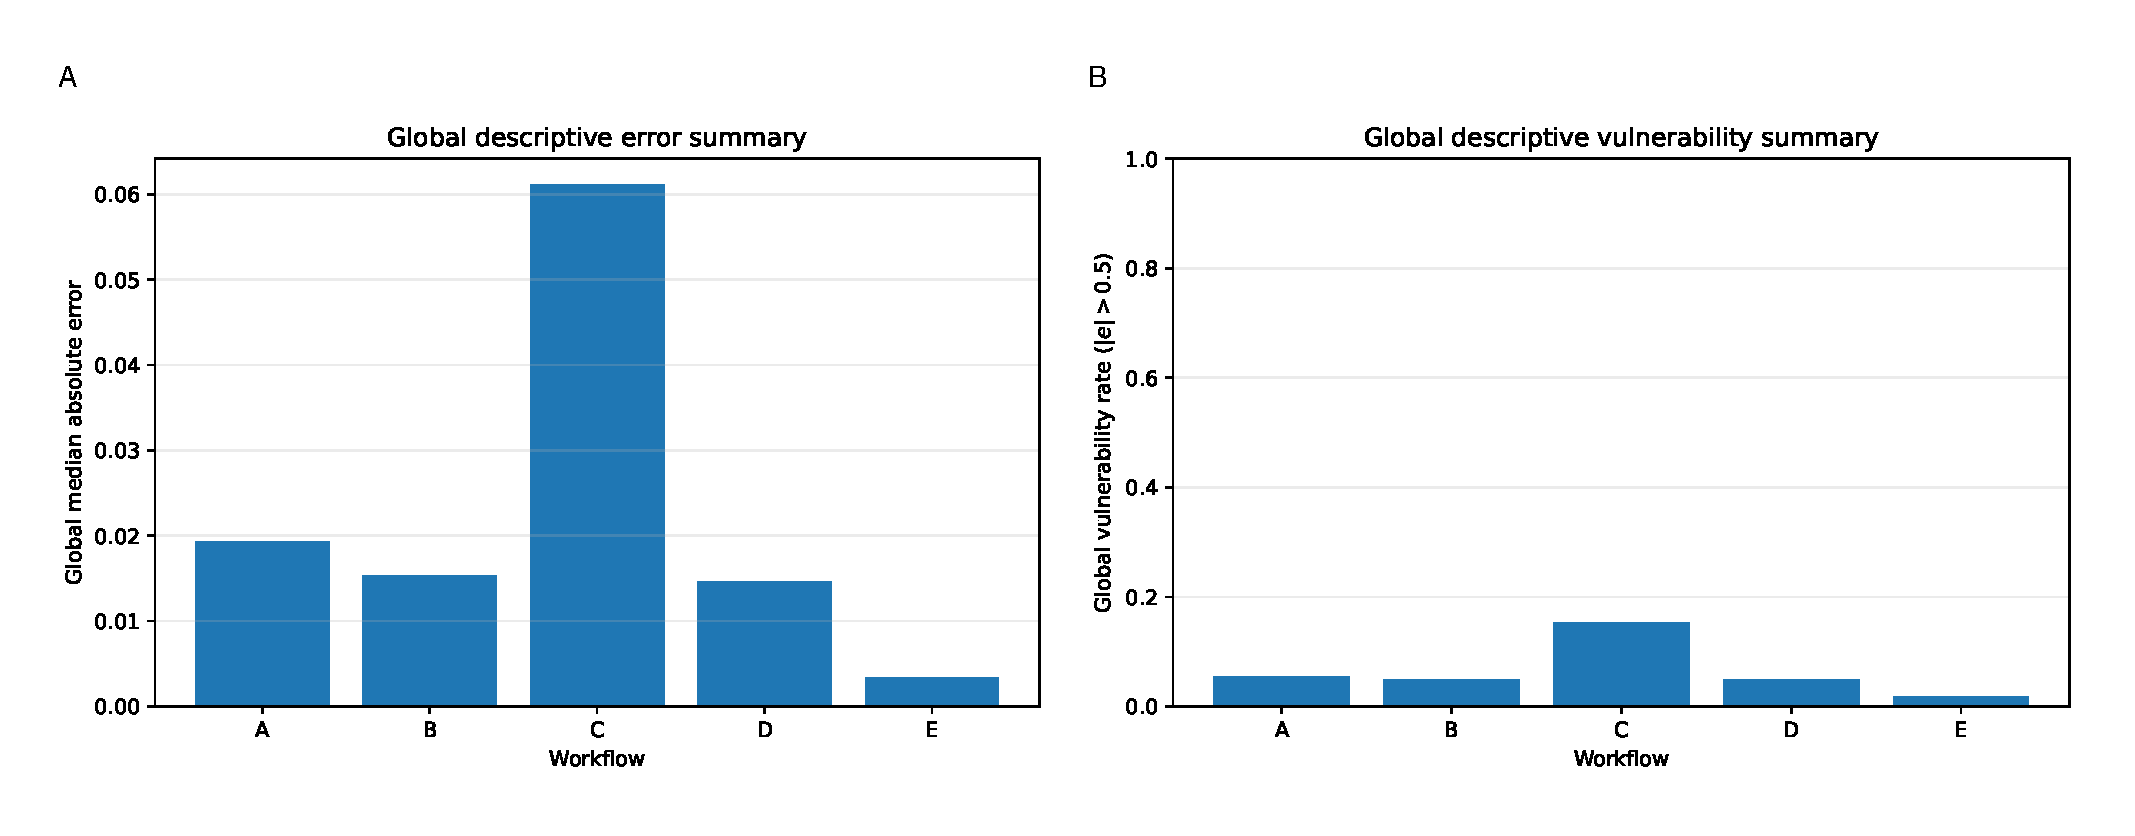
\includegraphics[width=0.88\linewidth]{figures/FIGURE_2_GLOBAL_CONTEXT.pdf}
\caption{Global pooled descriptive context for the primary comet-like experiment.}
\label{fig:global-context}
\end{figure}

\subsection{Cell-resolved error and vulnerability
landscape}\label{cell-resolved-error-and-vulnerability-landscape}

The 15 experimental cells show substantial variation in median absolute
error and in the fraction of evaluations exceeding the predefined
vulnerability threshold
(\texttt{\textbar{}e\textbar{}\ \textgreater{}\ 0.5}). The cell-resolved
median absolute-error landscape is shown in Fig. 3, and the
corresponding vulnerability landscape is shown in Fig. 4. For each cell,
\begin{figure}[htbp]
\centering
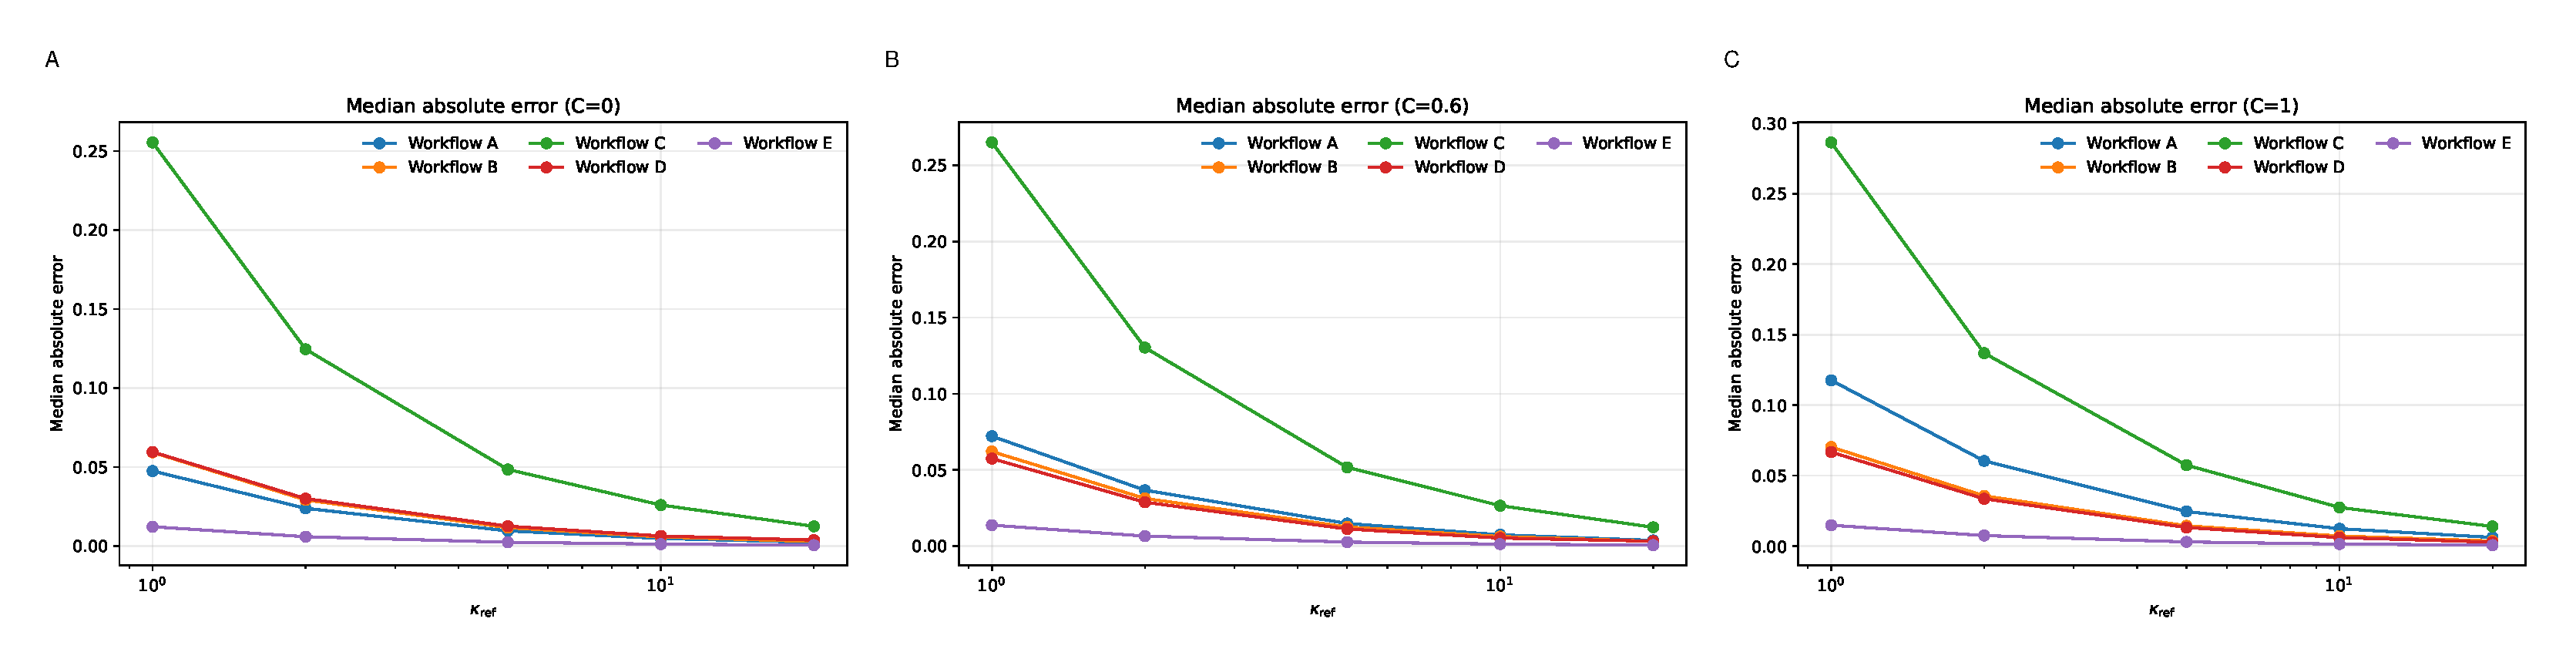
\includegraphics[width=0.88\linewidth]{figures/FIGURE_3_MEDIAN_ABS_ERROR_LANDSCAPE.pdf}
\caption{Cell-resolved median absolute-error landscape for the primary comet-like experiment.}
\label{fig:median-abs}
\end{figure}
\begin{figure}[htbp]
\centering
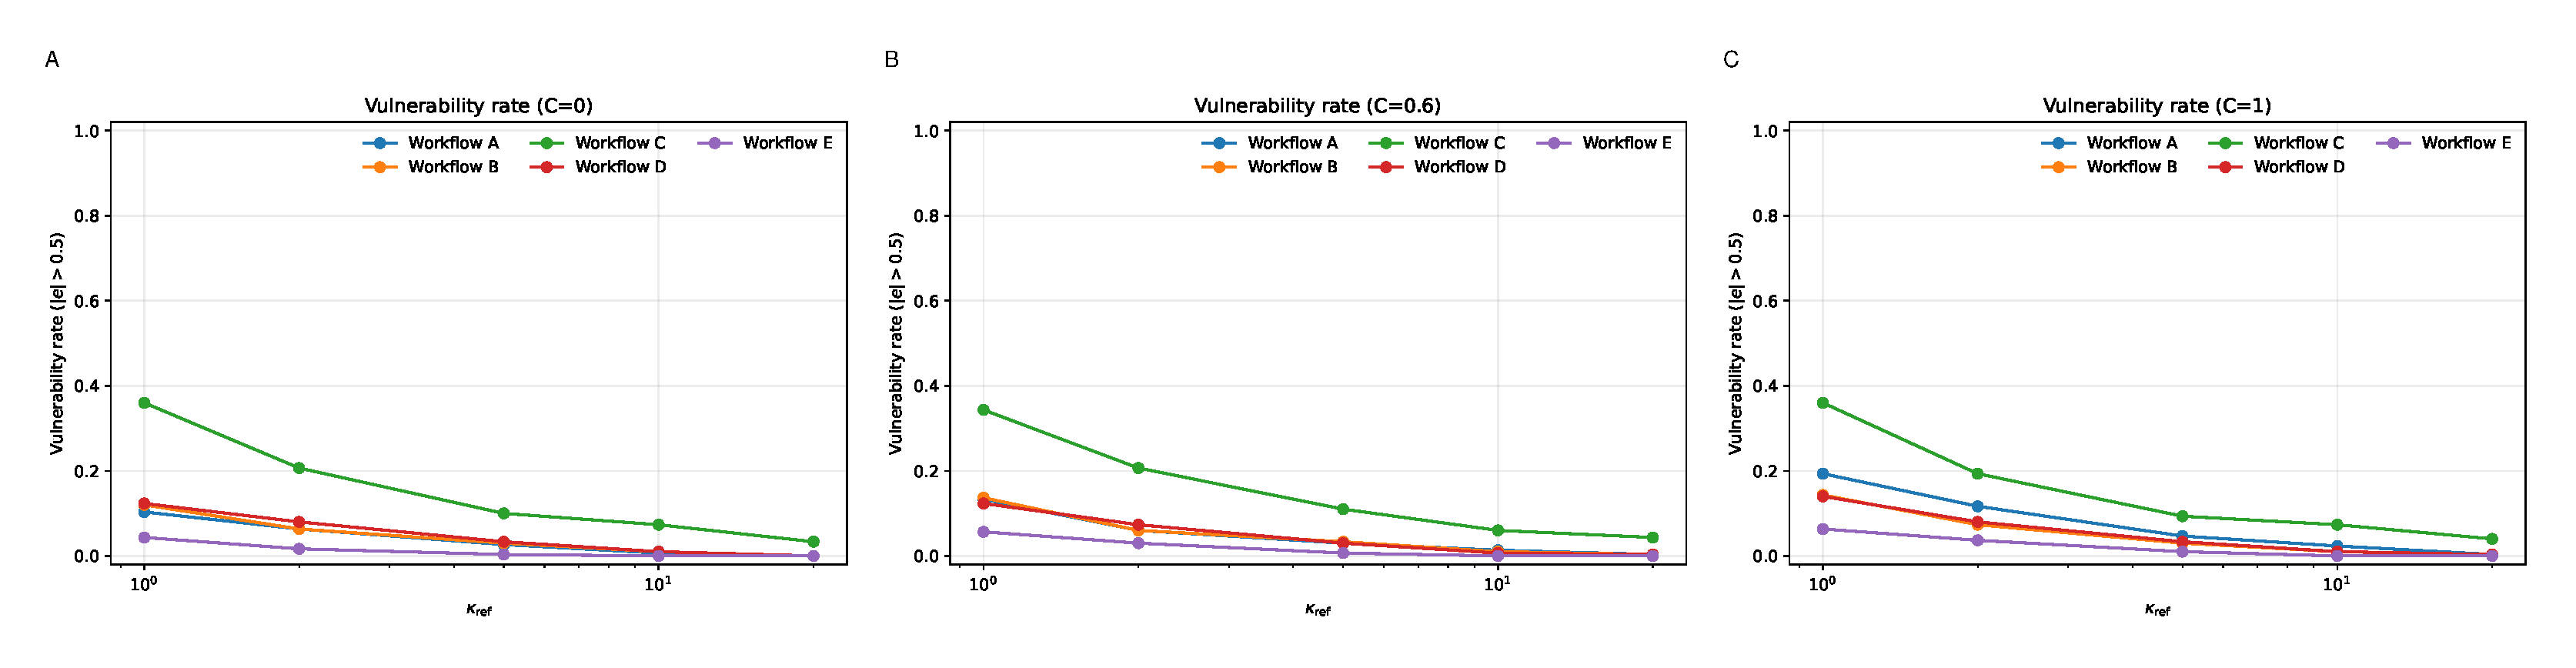
\includegraphics[width=0.88\linewidth]{figures/FIGURE_4_VULNERABILITY_LANDSCAPE.pdf}
\caption{Cell-resolved vulnerability landscape for the primary comet-like experiment at the primary threshold.}
\label{fig:vulnerability}
\end{figure}
the observed numerical span across workflows is:

\begin{itemize}
\tightlist
\item
  Reference contrast=1, C=0: median \textbar e\textbar{} spans 0.012--0.255 (lower
  endpoint: E; upper endpoint: C); vulnerability spans 4.3\%--36.0\%
  (lower endpoint: E; upper endpoint: C).
\item
  Reference contrast=2, C=0: median \textbar e\textbar{} spans 0.0060--0.125 (lower
  endpoint: E; upper endpoint: C); vulnerability spans 1.7\%--20.7\%
  (lower endpoint: E; upper endpoint: C).
\item
  Reference contrast=5, C=0: median \textbar e\textbar{} spans 0.0024--0.049 (lower
  endpoint: E; upper endpoint: C); vulnerability spans 0.3\%--10.0\%
  (lower endpoint: E; upper endpoint: C).
\item
  Reference contrast=10, C=0: median \textbar e\textbar{} spans 0.0012--0.026 (lower
  endpoint: E; upper endpoint: C); vulnerability spans 0.0\%--7.3\%
  (lower endpoint: E; upper endpoint: C).
\item
  Reference contrast=20, C=0: median \textbar e\textbar{} spans 6.177e-04--0.012
  (lower endpoint: E; upper endpoint: C); vulnerability spans
  0.0\%--3.3\% (lower endpoint: A,B,D,E; upper endpoint: C).
\item
  Reference contrast=1, C=0.6: median \textbar e\textbar{} spans 0.014--0.265 (lower
  endpoint: E; upper endpoint: C); vulnerability spans 5.7\%--34.3\%
  (lower endpoint: E; upper endpoint: C).
\item
  Reference contrast=2, C=0.6: median \textbar e\textbar{} spans 0.0066--0.130
  (lower endpoint: E; upper endpoint: C); vulnerability spans
  3.0\%--20.7\% (lower endpoint: E; upper endpoint: C).
\item
  Reference contrast=5, C=0.6: median \textbar e\textbar{} spans 0.0027--0.052
  (lower endpoint: E; upper endpoint: C); vulnerability spans
  0.7\%--11.0\% (lower endpoint: E; upper endpoint: C).
\item
  Reference contrast=10, C=0.6: median \textbar e\textbar{} spans 0.0013--0.027
  (lower endpoint: E; upper endpoint: C); vulnerability spans
  0.0\%--6.0\% (lower endpoint: E; upper endpoint: C).
\item
  Reference contrast=20, C=0.6: median \textbar e\textbar{} spans 6.540e-04--0.012
  (lower endpoint: E; upper endpoint: C); vulnerability spans
  0.0\%--4.3\% (lower endpoint: E; upper endpoint: C).
\item
  Reference contrast=1, C=1: median \textbar e\textbar{} spans 0.015--0.286 (lower
  endpoint: E; upper endpoint: C); vulnerability spans 6.3\%--36.0\%
  (lower endpoint: E; upper endpoint: C).
\item
  Reference contrast=2, C=1: median \textbar e\textbar{} spans 0.0075--0.137 (lower
  endpoint: E; upper endpoint: C); vulnerability spans 3.7\%--19.3\%
  (lower endpoint: E; upper endpoint: C).
\item
  Reference contrast=5, C=1: median \textbar e\textbar{} spans 0.0030--0.057 (lower
  endpoint: E; upper endpoint: C); vulnerability spans 1.0\%--9.3\%
  (lower endpoint: E; upper endpoint: C).
\item
  Reference contrast=10, C=1: median \textbar e\textbar{} spans 0.0015--0.027 (lower
  endpoint: E; upper endpoint: C); vulnerability spans 0.0\%--7.3\%
  (lower endpoint: E; upper endpoint: C).
\item
  Reference contrast=20, C=1: median \textbar e\textbar{} spans 7.387e-04--0.014
  (lower endpoint: E; upper endpoint: C); vulnerability spans
  0.0\%--4.0\% (lower endpoint: E; upper endpoint: C).
\end{itemize}

The corresponding cell-resolved values are listed below.

Complete cell-level values for all 75 cell--workflow groups, including
median absolute error, vulnerability rate, median signed error, and
realized contrast, are provided in Table S1.

\subsection{Signed-error behavior}\label{signed-error-behavior}

Median signed error is retained separately from absolute error to
distinguish error magnitude from direction. Figure S1 shows the frozen
signed-error curves across the three contamination levels. Complete
cell-level signed-error values are included in Table S1. Directional
structure is interpreted only together with error magnitude, workflow
information class, and the corresponding stress-grid cell.

\subsection{Reliability-boundary
framing}\label{reliability-boundary-framing}

The frozen grid is reported as a reliability landscape rather than as a
single global ranking. The cell-resolved summaries show that error
magnitude and vulnerability vary with both reference contrast and
contamination level \texttt{C}, and that the magnitude of separation
among workflows is not constant across the grid.

At this stage, the data support reporting: - where median absolute
errors remain small or become large; - where vulnerability rates become
nonzero or increase; - how those patterns shift across
reference contrast and \texttt{C}; - how signed-error behavior differs
from absolute-error behavior.

Interpretive explanations for why those patterns occur are reserved for
the Discussion.

\subsection{Paired uncertainty and
robustness}\label{paired-uncertainty-and-robustness}

Cluster-bootstrap uncertainty was evaluated with the 300 base sample
identities as the resampling units, preserving each identity's complete
cross-condition and cross-workflow block. The resulting intervals are
reported with the derived-analysis tables. Paired blind-workflow
contrasts confirm that the separations visible in the cell-resolved
landscape are condition dependent rather than reducible to a single
pooled ordering. In particular, the paired absolute-error difference
between workflows C and E is positive in all 15 tested cells, with the
95\% cluster-bootstrap interval above zero in every cell. The
corresponding A--E and B--E differences are also positive in all 15
cells, whereas A--B changes with contamination condition and some
low-contrast intervals include zero.

Paired stress-axis contrasts sharpen this condition-dependent
interpretation for the comet-like family. For contamination, 35 of 50
higher-\(C\) versus \(C=0\) contrasts had 95\% sample-identity
bootstrap intervals entirely above zero, 13 included zero, and two were
below zero; both negative intervals occurred for privileged-information
workflow D at \(\kappa_{\rm ref}=20\). Thus contamination
predominantly increased absolute error but not uniformly across all
workflow--contrast cells. In contrast, all 60 adjacent-\(\kappa\)
paired contrasts had intervals entirely below zero for
\(\Delta|e|=|e|_{\kappa_{\rm high}}-|e|_{\kappa_{\rm low}}\),
indicating lower absolute error at each successive tested
reference-contrast level across all workflows and contamination
settings.

Threshold sensitivity confirms that the numerical location of a
threshold-defined boundary depends on the operational cutoff. The
primary \(\tau=0.5\) analysis exactly reproduces the predefined
boundary table below. At \(\tau=0.4\), the A boundary at \(C=1\) moves
from \(\kappa_{\rm ref}=5\) to 10; at \(\tau=0.6\), the E boundary at
\(C=0.6\) moves from 2 to 1 while the A--D primary boundaries are
unchanged. More stringent or permissive cutoffs produce larger shifts.
Continuous error surfaces are therefore treated as primary evidence and
threshold boundaries as an operational summary.

Excluding the three Workflow-E evaluations with optimizer
\texttt{success=False} changes the affected cell median absolute errors
by at most \(9.02\times10^{-5}\), indicating no material effect on the
reported reliability landscape.

\subsection{Pre-registered compact-PSF extension}
\label{results-compact-psf-extension}

The second family contains 300 base identities and 18,000 workflow
evaluations across 60 condition--workflow groups. All 40 paired
contamination contrasts comparing \(C=0.6\) or 1 with \(C=0\) had
95\% bootstrap intervals above zero. Of 48 adjacent-\(\kappa\)
contrasts, 32 had intervals below zero; the remaining 16 were all
\(C=0\) clean cells, where error was already at the numerical floor.
Restricting the comparison to contaminated cells therefore gives 32 of
32 adjacent-\(\kappa\) intervals below zero.

Workflow-relative structure also differed from the comet-like family.
Within contaminated compact-PSF cells, workflow E had lower paired
absolute error than A, B, and C throughout the tested grid; A had lower
paired error than B and C, whereas B--C intervals included zero
throughout those cells. The E result is interpreted as a
family-specific model-match effect because the source truth is itself a
circular Gaussian, not as evidence of universal workflow superiority.
Threshold sensitivity placed operational vulnerability mainly in the
low-contrast, high-contamination region; by
\(\kappa_{\rm ref}\geq5\), vulnerability was essentially absent
even at \(\tau=0.25\), apart from one 1/300 event for workflow C at
\(\kappa_{\rm ref}=5,C=1\).

\section{Discussion}\label{discussion}

\subsection{Reliability is a landscape rather than a single aggregate
score}\label{reliability-is-a-landscape-rather-than-a-single-aggregate-score}

The frozen AMPV V2 results are most naturally interpreted as a
reliability landscape over reference contrast and contamination level,
rather than as a single global ordering of workflows. The global
summaries are:

\begin{itemize}
\tightlist
\item
  Workflow A: global median \textbar e\textbar=0.019; global
  vulnerability=5.5\%; global median signed e=0.012.
\item
  Workflow B: global median \textbar e\textbar=0.015; global
  vulnerability=4.8\%; global median signed e=0.0057.
\item
  Workflow C: global median \textbar e\textbar=0.061; global
  vulnerability=15.3\%; global median signed e=8.852e-04.
\item
  Workflow D: global median \textbar e\textbar=0.015; global
  vulnerability=5.0\%; global median signed e=0.0025.
\item
  Workflow E: global median \textbar e\textbar=0.0034; global
  vulnerability=1.8\%; global median signed e=8.213e-04.
\end{itemize}

These aggregate values are useful for orientation, but they pool cells
whose error and vulnerability behavior can differ materially. For that
reason, the cell-resolved surfaces remain the primary evidence for
identifying stable and vulnerable operating regions.

Across the frozen reference-contrast grid, median absolute error and
vulnerability generally decline as reference contrast increases for all
workflows and contamination levels. The strongest residual vulnerability
occurs for workflow C at low contrast, while workflow E reaches low
vulnerability at lower tested contrast levels. The complete
workflow-by-contamination monotonic trend listing is provided in
Supplementary Note S1.

This pattern supports the methodological use of AMPV as a
boundary-mapping framework: the relevant question is not only whether
two workflows differ on average, but also whether their error behavior
remains stable as the controlled stressors move across the grid.

\subsection{Contamination changes the shape of the reliability
surface}\label{contamination-changes-the-shape-of-the-reliability-surface}

At fixed reference contrast, contamination modifies the observed error
and vulnerability patterns in a workflow-dependent manner. The effect is
strongest in the low-contrast regime and is not uniformly monotonic for
every workflow--contrast combination. Consequently, contamination cannot
be summarized independently of reference contrast or information class.
The complete cell-by-cell contamination trend listing is provided in
Supplementary Note S2.

\subsection{A threshold-based view exposes operational
boundaries}\label{a-threshold-based-view-exposes-operational-boundaries}

Using the predefined vulnerability threshold \textbar e\textbar{}
\textgreater{} 0.5, the lowest tested reference contrast at which
vulnerability is \textless=5\% is summarized below.

\begin{longtable}[]{@{}lrrr@{}}
\toprule\noalign{}
Workflow & C=0 & C=0.6 & C=1 \\
\midrule\noalign{}
\endhead
\bottomrule\noalign{}
\endlastfoot
A & 5 & 5 & 5 \\
B & 5 & 5 & 5 \\
C & 20 & 20 & 20 \\
D & 5 & 5 & 5 \\
E & 1 & 2 & 2 \\
\end{longtable}

This boundary table should be interpreted only within the tested grid.
\cite{ref6} It does not imply behavior between untested reference-contrast levels,
and it should not be extrapolated beyond the frozen contamination range.

\subsection{Information class matters for
interpretation}\label{information-class-matters-for-interpretation}

The frozen production metadata distinguish workflow D as the
oracle-diagnostic information class, whereas the remaining workflows are
blind. Therefore, numerical differences involving D should not be
interpreted as if all workflows operate under the same information
constraints. Workflow D is used as a diagnostic reference for what
becomes possible with privileged information rather than as a directly
interchangeable blind estimator.

This distinction is methodological rather than cosmetic: reliability
claims should remain conditional on the information available to a
workflow.

\subsection{Signed error and absolute error answer different
questions}\label{signed-error-and-absolute-error-answer-different-questions}

The analysis retains both absolute and signed error. Absolute error
describes magnitude and is therefore used for vulnerability mapping,
whereas signed error preserves direction. The signed-error figure is
retained as supplementary material so that directional structure remains
inspectable without replacing the primary magnitude-based reliability
view.

A directional pattern should not be described as improved or degraded
performance solely from its sign. The interpretation must remain tied to
error magnitude, information class, and the relevant cell of the stress
grid.

\subsection{Cross-family structure is reproducible but
task-dependent}\label{cross-family-structure}

The extension does not reproduce a fixed workflow ordering, nor was
that the pre-registered transfer criterion. Across both controlled
families, increasing tested reference contrast is associated with lower
paired absolute error wherever nontrivial error remains, compound
contamination changes the reliability landscape, and matched identities
resolve workflow-dependent structure. However, the detailed
contamination response, workflow ordering, and vulnerability boundaries
differ between the comet-like and compact-PSF tasks.

This heterogeneity is methodologically informative. In the comet-like
family, contamination is not uniformly monotonic and A--B behavior
changes with contamination. In the compact-PSF family, all tested
contamination contrasts are adverse and the Gaussian-fitting workflow
benefits from direct model match. AMPV should therefore be interpreted
as a framework for estimating task-conditional reliability structure,
not for assigning a task-independent score or universal workflow
ranking.

\subsection{What the present experiment does and does not
establish}\label{what-the-present-experiment-does-and-does-not-establish}

The study contains two frozen single-fidelity controlled experiments.
The original canonical comet-like production establishes the tested
reliability landscape for \texttt{COMET\_LIKE\_PRIMARY}, the five
reference-contrast levels, the three contamination levels, and workflows
A--E under its V2-native matched stochastic design. The separately
versioned compact-PSF extension establishes the corresponding tested
landscape for \texttt{COMPACT\_PSF\_PRIMARY} with blind workflows
A, B, C, and E. Neither production is retroactively redefined by the
other.

It does \textbf{not} by itself establish fidelity dependence across
multiple simulation fidelities. \cite{ref5} Any manuscript claim about
fidelity dependence would require additional, explicitly authorized
multi-fidelity experiments or must be framed as future work rather than
as a result of the present production.

Likewise, the synthetic environment provides controlled access to ground
truth and reproducible perturbations, but behavior on observational
datasets outside the tested validation domain still requires external
validation \cite{ref5,ref6}. The value of the framework is therefore
methodological: it provides a reproducible way to expose where a
workflow remains stable, where it becomes vulnerable, and which
controlled stressors are associated with those changes.

\subsection{Relationship between AMPV and
CAPS}\label{relationship-between-ampv-and-caps}

AMPV and CAPS are kept conceptually distinct. AMPV is the general
validation methodology developed around reliability mapping and boundary
analysis, whereas CAPS is one controlled synthetic implementation
environment that can support such validation experiments. The present V2
production is independently realized and canonically frozen within the
AMPV V2 project tree; CAPS V1 production outputs are not used as the
present canonical evidence.

This framing avoids treating AMPV as merely a renamed workflow or a
simple continuation of the earlier ranking study.

\subsection{Limitations and next validation
steps}\label{limitations-and-next-validation-steps}

The present results are bounded by the tested grids, the two controlled
synthetic task families, the current fidelity level, and their synthetic
forward-model assumptions. The current analysis also uses a predefined vulnerability
threshold of 0.5; alternative thresholds may change the location of
threshold-defined boundaries even when the underlying continuous error
surface is unchanged. The explicit sensitivity analysis confirms this
dependence and therefore supports interpreting the threshold table as an
operational diagnostic rather than a physical transition.

Useful next validation steps include testing additional fidelity levels,
expanding the stress grid where transitions appear sharp, and evaluating
the framework with observationally anchored injections, real-image test
sets, or independently implemented community pipelines.
\cite{ref6} \cite{ref5} These extensions should be run as new, versioned
experiments rather than retrofitted into the frozen canonical release.

Literature-dependent context is limited to the source-level-audited
references. Interpretation of the present numerical results remains
separated from prior-art context and is restricted to the frozen tested grids, information classes, and single-fidelity production records.

\section{Conclusions}\label{conclusions}

The primary frozen AMPV V2 comet-like experiment demonstrates a
reproducible way to evaluate photometric workflows as a reliability
landscape rather than as a single aggregate ranking. Across 300 base
stochastic identities, 4,500 condition-specific scene instances, and
22,500 workflow evaluations, that primary analysis retains cell-resolved
error magnitude, signed error, vulnerability, workflow information
class, and matched-scene provenance across the tested reference-contrast
and contamination grid.

The results support boundary-oriented reporting: workflow behavior
varies across the frozen stress grid, and pooled summaries alone do not
preserve the full structure of those changes. The common-random-number
design follows an established simulation-comparison strategy
\cite{ref7}, while reproducibility and traceability in the present study
are provided by the audited canonical release chain.

The pre-specified, internally frozen extension broadens the evidence from one to two
materially distinct controlled synthetic photometric task families.
Both recover cell-resolved stress-dependent reliability structure, while
their workflow-relative behavior and operational boundaries differ.
This supports task-conditional reliability mapping rather than a
universal ranking interpretation.

The present evidence is intentionally bounded. It is a single-fidelity
synthetic study and therefore does not establish multi-fidelity
dependence. More generally, the synthetic evidence should not be assumed
to generalize unchanged to observational datasets outside the tested
validation domain \cite{ref5,ref6}. Those questions require separately
versioned validation experiments rather than reinterpretation of the
frozen release.

Within that scope, AMPV provides a methodology for moving from average
workflow comparison toward explicit mapping of stable and vulnerable
operating regions under controlled perturbation.
